\chapter{実装}
\label{chap:zissou}

本章では第\ref{chap:sekkei}章で述べたシステムの設計を受け、DrawWikiの実装について述べる。

\newpage

\section{アプリケーション構成}
DrawWikiはWebアプリケーションとして実装されているためHTML5とSVG1.1に準拠したブラウザがあれば、
OSやデバイスに依存せず利用することができる。本アプリケーションの構成は以下の図の通りである。

\begin{figure}[htbp]
    \begin{center}
        \fbox {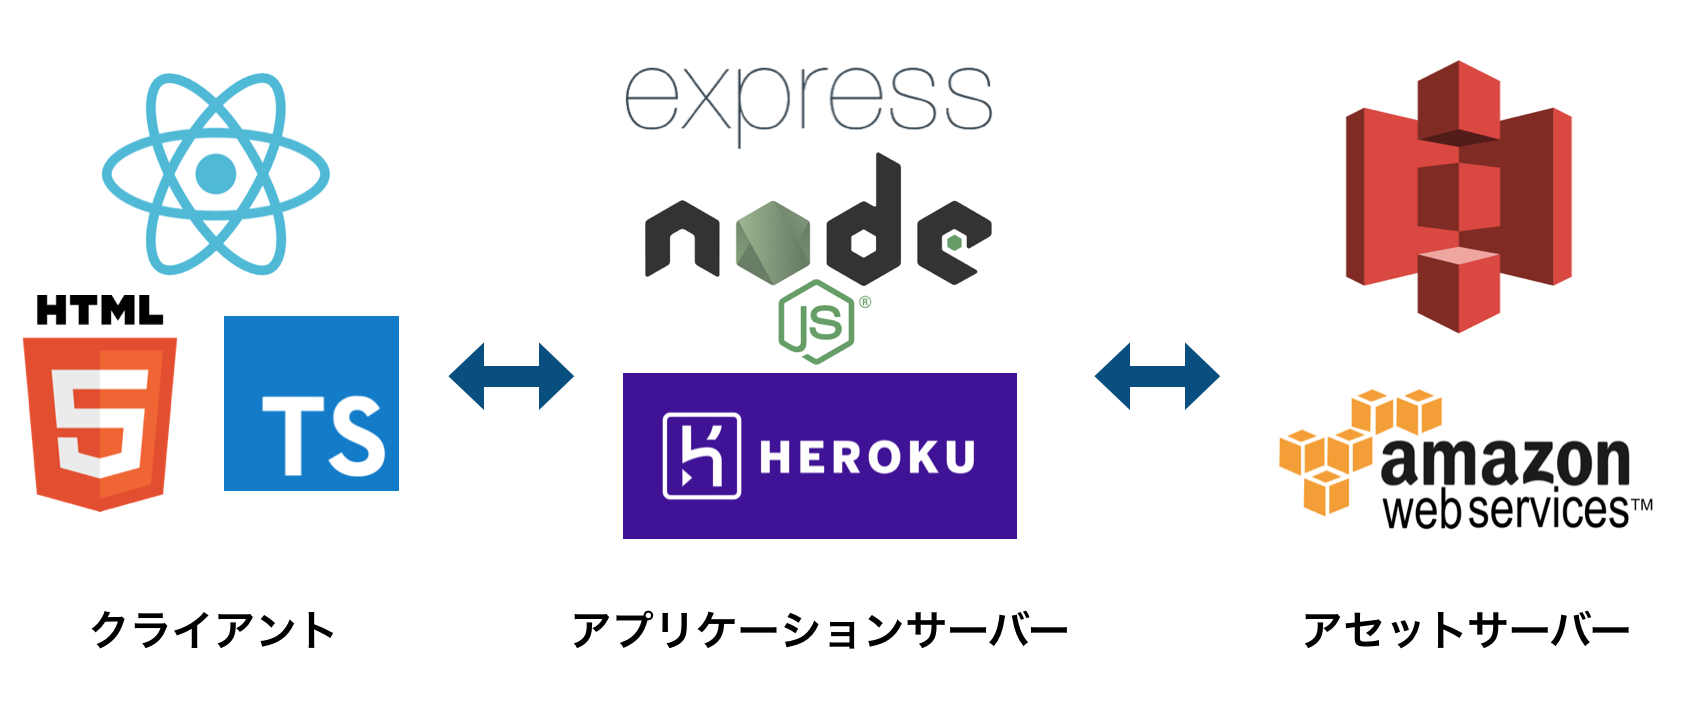
\includegraphics[width=110mm]{images/application.png}} \end{center}
    \caption{アプリケーションの構成}
\end{figure}

\section{クライアントサイド}
実際に手書きメモ・イラストの作成や関連画像の表示を行うクライアントサイドのプログラムはHTML\footnote{https://developer.mozilla.org/ja/docs/Web/HTML}と
javascript\footnote{https://developer.mozilla.org/ja/docs/Glossary/JavaScript}によって実装されている。
開発にはJavascriptにコンパイル可能な漸進的型付け言語TypeScript\footnote{https://www.typescriptlang.org/}を用いている。

\subsection{手書きデータの取得}
DrawWikiにおいて指やスタイラスの操作から生じる座標等の手書きデータをPointerEvent API\footnote{https://developer.mozilla.org/ja/docs/Web/API/PointerEvent}によって取得している。
このAPIはTouchEventやMouseEventと異なりタッチやマウスだけでなくスタイラスを含めたあらゆるユーザー入力を透過的に扱うことが可能で(図\ref{pevent})、
また主要なブラウザに全て実装されているためあらゆるプラットフォーム・デバイスから利用できる。

\begin{figure}[htbp]
    \begin{center}
        \fbox {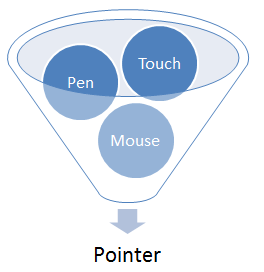
\includegraphics[width=50mm]{images/pevents.png}} \end{center}
    \caption{PointerEvent APIの概要} \label{pevent}
\end{figure}

\subsection{手書きデータの描画}
DrawWikiはミリ秒単位の頻度で発生するPointerEventから動的に手書きストロークを生成し、
選択された要素をグループ化した上でハイパーリンクを追加する等のSVGに対する複雑な操作を行っている。
一般的にSVGの操作はHTMLと同じくDOMインターフェース(appendChildやremoveChild、insertBefore等)を用いて行うが、
操作の度にSVGのDOMにアクセスすることは処理の複雑化と描画パフォーマンスの低下を招く。
そこでDrawWikiでは実際に表示されているSVGのDOMとは別に、プログラム上で仮想的なDOMを構築し、
要素の属性変更やハイパーリンクの埋め込み等の処理を仮想DOM上で行い、その操作が完了した段階で
実際のDOMとの差分をDispatchするという手法を用いている。
これによって処理の簡略化と描画パフォーマンスの向上を実現している。仮想DOM構築と実DOMへの反映は
ViewライブラリのReact\footnote{https://ja.reactjs.org/}を利用している。

\subsection{debounceされた更新処理}
DrawWikiは手書きメモ・イラストが編集され変更が生じる度に自動でデータを上書きし保存するが、画面上で指やスタイラスペンを動かしている間は
常にPointerEventが発生し続けているため、この頻度で変更をアップロードするとサーバー側の処理能力を超えてしまう。
そこでEvent発生後にタイマーをセットし、2秒経過した段階でアップロード処理を行うdebounce機能を実装した。このタイマーは新しいEventが
発生する度にリセットされるため、ペンを置いてしばらく、つまり最後のEventから2秒間新たなEventが発生しないことが確定してからアップロード処理が行われる。
これによりアプリケーションサーバーやアセットサーバーに過大な負荷を与えることなく更新処理を行うことができる。


\subsection{リンク付要素の視覚的表現}

\begin{figure}[htbp]
    \begin{center}
        \fbox {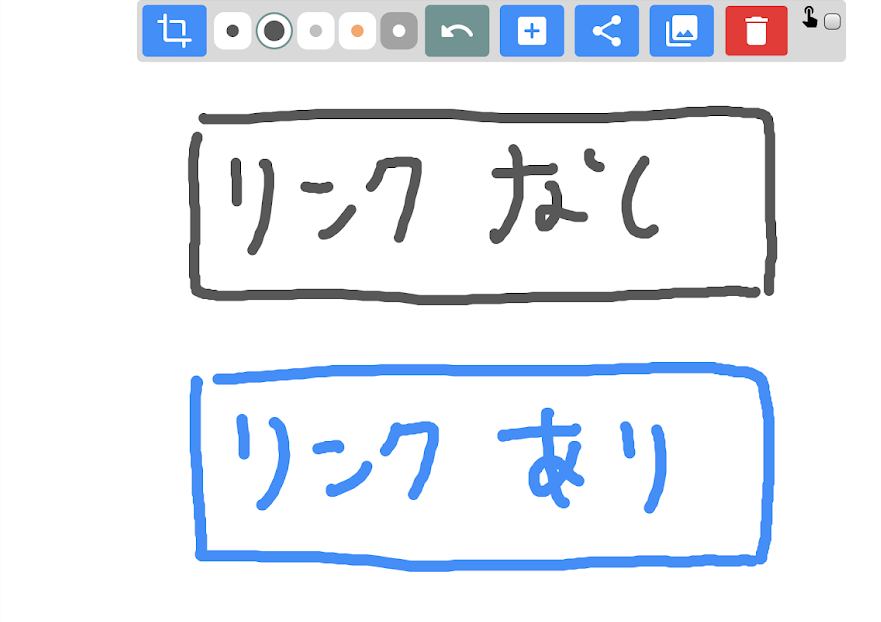
\includegraphics[width=110mm]{images/linkedstyle.png}} \end{center}
    \caption{リンクされていない要素(上)とされている要素(下)} \label{linkedelm}
\end{figure}

関連画像ビューにはリンクしている手書きメモ・イラストのサムネイルが表示される。
そのサムネイルを選択するとリンクされているキャンバス内の要素が視覚的に変化し、対応関係が強調表示される(図\ref{linkedelm})。
SVGはその仕様上CSS\footnote{https://developer.mozilla.org/ja/docs/Web/CSS}を適用することも可能なため
この視覚効果はCSSとCSS @keyframes\footnote{https://developer.mozilla.org/ja/docs/Web/CSS/@keyframes}を組み合わせることで実現している。

\section{サーバーサイド}
サーバーサイドはアプリケーションサーバーとアセットサーバーとで構成されている。

\subsection{アプリケーションサーバー}
DrawWikiはNode.js\footnote{https://nodejs.org/}上で動作するWebアプリケーションとして実装されている。
HTTPリクエストを処理するWebアプリケーションフレームワークとしてExpress\footnote{https://expressjs.com/}を用い、
そのホスティング環境としてBaaS(Backend-as-a-Service)の一つであるHeroku\footnote{https://www.heroku.com/}を利用している。

\subsubsection{手書きメモ・イラストのアップロード処理}
クライアントは作成した手書きメモ・イラストを"multipart/form-data"形式でエンコーディングして送信し、アプリケーションサーバーは
そのデータをPOST通信で受け取る。その後は自動生成されるメタデータ(ソースコード\ref{code:metadatajson})とともにデータをアセットサーバーにアップロードする。

また既存のメモ・イラストやメタデータの読み取り、更新、削除等の操作はREST原則\cite{Fielding2000ArchitecturalSA}
に基づいたルーティングによって処理される。

\subsubsection{メタデータの構成}
手書きメモ・イラストの本体データとは別に、以下のようなメタ情報を管理するためにDrawWikiではメタデータファイルも取り扱う。
\begin{itemize}
    \item メモ・イラストの作成者
    \item 最終更新日時
    \item 引用している/引用されているメモ・イラストのリスト
\end{itemize}

\begin{lstlisting}[caption=メタデータの概要, label=code:metadatajson]
    export type HyperIllust = {
    id: string; //手書きメモ・イラストのID
    sourceKey: string; //本体SVGファイルのKey
    sourceURL: string;  //本体SVGファイルのURL(フルパス)
    size?: number;  //ファイルサイズ
    linkedList?: string[];  //リンクされているメモ・イラストのIDリスト
    linkedByList?: string[];    //この画像をリンクしているメモ・イラストのIDリスト
    createdAt: DateLike;    //作成日時
    updatedAt: DateLike;    //更新日時
    owner: string;  //作成者の名前
    };
\end{lstlisting}

\subsection{アセットサーバー}
アプリケーションサーバーはステートレスなプロセスとして実行されるため、変数やファイル等を保存し永続化する仕組みをもたない。
ファイルとしてのメモ・イラストやメタデータを保存するためDraWikiはアセットサーバーとして
クラウドストレージであるAWS S3\footnote{https://aws.amazon.com/jp/s3/}を利用している。
アップロードされたメモ・イラストはDrawWiki以外のWebサイトからも閲覧・再利用できるように、ACL(Access-Control-List)を
公開読み取り("public-read")に設定している。またアセットサーバー自体もオリジン間リソース共有\footnote{https://developer.mozilla.org/ja/docs/Web/HTTP/CORS}
を有効化している。
